We introduce $T$-equivariant cohomology and some classical results about the
$T$-equivariant cohomology of smooth projective toric varieties.

\subsection{Basic properties}
Let $T$ be a complex torus. The equivariant cohomology ring $H_T^*(X)$ of a $T$-space $X$ is
defined as the singular cohomology of the Borel construction $X\times_T ET$,
where $ET$ is a contractible space on which $T$ acts freely. Such a space
always exists and is unique up to homotopy equivalence, see \cite{hatcher}.

\begin{example}
	We can identify $U(n)$ as those complex matrices preserving
	the standard Hermitian form on $\C^n$. The group $U(n)$ acts on $S^{2n-1}$ transitively and the stabilizer of the point $(1,0,\ldots,0)$ is $U(n-1)$.

	Therefore there is a canonical action of $U(1) = U(n)/U(n-1)$ acting as scalar matrices on $S^{2n-1}$ inherited from the action on $U(n)$. None of these odd dimensional spheres are contractible, but $S^\infty$ is contractible. In particular $EU(1) = S^\infty$ and \begin{align*}
		BU(1) = S^\infty/U(1) = \C\P^\infty
	\end{align*}
	Therefore \begin{align*}
		H^*_{U(1)}(pt) = H^*(\C\P^\infty) = \Z[t]
	\end{align*} where $t$ is the first Chern class of the tautological line bundle and $\deg t = 2$. The classifying space $B\C^*$ of an algebraic torus is
	homotopy equivalent to that of its maximal compact subgroup, so \begin{align*}
		H^*_{\C^*}(pt) = H^*(\C\P^\infty) = \Z[t]
	\end{align*} as well.
\end{example}

\begin{example}
	In general, $H_T^*(\text{pt})$ identifies with the representation ring of $T$. \begin{align*}
		BT \cong \prod_{\rank T} \C\P^\infty \\
		H_T^*(pt) = H^*(BT) = \Z[t_1,\ldots,t_{\rank T}]
	\end{align*}

	Given a representation $V$ of $T$,
	we can form a vector bundle on the classifying space whose
	total Chern class is equal to the class of $V$ in the representation ring, see \cite{huybrechts}.
\end{example}

Here are some important properties to know about equivariant cohomology:
\begin{enumerate}
	\item functoriality;
	\item a ring structure;
	\item excision;
	\item the Mayer-Vietoris sequence;
	\item the Künneth formula;
	\item the Leray spectral sequence;
	\item for smooth orientable $X$, Poincaré duality; and
	\item existence of Chern classes,
\end{enumerate}
where all subsets and maps are assumed to be equivariant. Let $\Lambda = H_T^*(\text{pt})$. The ring $H^*_T(X)$ is a module over $\Lambda$ via the map $X \to \text{pt}$.


\subsection{Invariant curves}
This section explores some key topological ideas underpinning equivariant localization. Theorem \ref{thm:slice} provides the local structure near orbits and simplifies the analysis of tangent spaces at fixed points. See \cite{fulton-anderson} for a detailed discussion of the results in this section.

\begin{theorem}[Slice theorem]
	\label{thm:slice}
	Let $X$ be a nonsingular complex algebraic variety.
	\begin{enumerate}
		\item Suppose $K$ is a compact Lie group acting on $X$, with an orbit $O = K \cdot x \subseteq X$. Then there is a $K$-invariant open neighborhood $U \subseteq X$ of $O$ which is equivariantly isomorphic to an open neighborhood of the zero section in the normal bundle $N_{O/X}$.

		\item Suppose $X$ is affine, and $G$ is a reductive group acting on $X$, with a closed orbit $O = G \cdot x$. Then there is a $G$-equivariant étale neighborhood $U \to X$ of $O$ which is equivariantly isomorphic to an étale neighborhood of the zero section of the normal bundle $N_{O/X}$.
	\end{enumerate}
\end{theorem}
\begin{lemma}
	Let $G$ be a connected reductive linear algebraic group (or compact connected Lie group) acting on a nonsingular algebraic variety $X$, with a fixed point $p \in X^G$. The point $p$ is isolated if and only if the trivial representation does not occur in $T_p X$.
\end{lemma}
When $G$ is a torus and $\dim X = n$, the lemma reads that $p\in X^T$ is isolated if and only of $c_n^T(T_pX) \neq 0$.
\begin{proof}
	By the slice theorem, we can reduce to the case where $X = V$ is a representation of $G$, and $p = 0$ is the origin. In this case, for any representation $V$ of a connected group, the origin $0 \in V$ is an isolated fixed point if and only if $V$ contains no copy of the trivial representation.
\end{proof}

The \( T \)-invariant curves in a variety \( X \) are important invariants. In particular, they determine the image of the restriction homomorphism
\[
	\iota^* : H_T^*X \to H_T^*X^T.
\]
First, we introduce notation and basic facts about such curves. Suppose \( T \) acts on \( \mathbb{P}^1 \) by distinct characters \( \chi_1 \) and \( \chi_2 \), so the fixed points are \( 0 = [1, 0] \) and \( \infty = [0, 1] \). Writing \( \chi = \chi_2 - \chi_1 \), we have
\[
	T_0\mathbb{P}^1 = \mathbb{C}_\chi \quad \text{and} \quad T_\infty\mathbb{P}^1 = \mathbb{C}_{-\chi}.
\]
More generally, if \( T \) acts on a nonsingular curve \( C \) with \( C^T = \{p, q\} \), then there is an equivariant isomorphism \( C \cong \mathbb{P}^1 \) sending \( p \) to \( 0 \) and \( q \) to \( \infty \). The action of $T$ on the open set $\C^*\subset\P^1$ determines up to sign \( \pm\chi \) the \emph{character of \( T \) acting on \( C \)}.

\begin{proposition}
	Let \( T \) act on an \( n \)-dimensional nonsingular algebraic variety \( X \), and let \( p \in X^T \) be an isolated fixed point, so the tangent weights \( \chi_1, \dots, \chi_n \) on \( T_p X \) are all nonzero.
	\begin{enumerate}
		\item If no two characters at \( p \) are parallel, then there are finitely many \( T \)-curves in \( X \) through \( p \). In fact, there are \( n \) such curves, all nonsingular at \( p \), with characters \( \chi_1, \dots, \chi_n \).
		\item If two characters have the same direction, then there are infinitely many \( T \)-curves through \( p \).
		\item If two characters have opposite directions, then there are infinitely many \( T \)-curves through any \( T \)-invariant neighborhood of \( p \).
	\end{enumerate}
\end{proposition}
Understanding the tangent weights at fixed points is crucial for the study of equivariant cohomology. The following theorem is a key result in this direction.
\begin{theorem}[Localization Theorem]
	Consider a $d$-dimensional nonsingular variety $X$ with finitely many fixed points. Let
	\[
		c = \prod_{p \in X^T} c_d^T(T_p X) \in \Lambda,
	\]
	and let $S \subseteq \Lambda$ be a multiplicative set containing $c$ (which is nonzero, since all fixed points are isolated). Assume there are $m \leq \#X^T$ classes in $H^*_T X$ restricting to a basis of $H^* X$.

	Then $m = \#X^T$, the homomorphisms
	\[
		S^{-1} H^*_T X \xrightarrow{S^{-1} l^*} S^{-1} H^*_T X^T \quad \text{and} \quad S^{-1} H^*_T X^T \xrightarrow{S^{-1} l_*} S^{-1} H^*_T X
	\]
	are isomorphisms, and $l^*: H^*_T X \to H^*_T X^T$ is injective.
\end{theorem}

\subsection{Localization formula}
At its core, the equivariant localization formula, introduced by Atiyah-Bott and Berline-Vergne, arises from the principle that, under certain conditions, integrals over a compact space with a torus action can be “localized” to the fixed points of the action. This idea can be traced back to the stationary phase approximation in physics, where integrals are approximated by contributions from critical points. In the equivariant cohomology setting, the fixed points of the torus action play a similar role. We refer to \cite{fulton-anderson} for a detailed discussion.

\begin{theorem}
	[Atiyah-Bott, Berline-Vergne]
	Let $X$ be a $d$-dimensional nonsingular compact algebraic variety with finitely many fixed points. Then
	\[
		\rho_*(u) = \sum_{p \in X^T} \frac{u|_p}{c_d^T(T_p X)}
	\]
	for any class $u \in H^*_T X$.
\end{theorem}

\begin{example}
	Consider $T = \mathbb{C}^*$ acting on $\mathbb{P}^2$ by the characters $0, t, 2t$. The fixed points are the usual coordinate points $p_1, p_2, p_3$. For $u \in H^*_T \mathbb{P}^2$, let $u_i = u|_{p_i}$. Near $p_1$ say, we have coordinates $y/x, z/x$ and therefore the weights of the $T$-action on $T_{p_1} \mathbb{P}^2$ are $t, 2t$. As a whole, the integration formula says
	\[
		\rho_*(u) = \frac{u_1}{2t^2} + \frac{u_2}{-t^2} + \frac{u_3}{2t^2} = \frac{u_1 - 2u_2 + u_3}{2t^2}.
	\]

	This must be a class in $\Lambda = \mathbb{Z}[t]$, so the integration formula implies a \textit{divisibility condition} relating the restrictions to the three fixed points: $2t^2$ must divide the polynomial $u_1 - 2u_2 + u_3$.
\end{example}

When computing via localization, it is often convenient to represent the fixed points of $X$ as the vertices of a graph, with edges connecting vertices when the corresponding fixed points are connected by a $T$-invariant curve. This graph is called the \textit{moment graph} of $X$, and coincides precisely with the image of the invariant curves in $X$ under the moment map.

The image of a class under the restriction
\[
	H^*_T X \hookrightarrow H^*_T X^T
\]
is given by labeling the vertices of the moment graph with characters. See \cite{hhh} for detailed discussion of these moment graphs, also known as GKM graphs due to work by Goresky, Kottwitz, and MacPherson \cite{gkm}.

\begin{theorem}
	[GKM]Let \( X \) be a nonsingular variety with \( X^T \) finite, and assume \( H_T^*X \) is free over \( \Lambda \). Suppose that for each \( p \in X^T \), the weights on \( T_pX \) are relatively prime. Then a tuple
	\[
		(u_p)_{p \in X^T} \in H_T^*X^T
	\]
	lies in the image of \( \iota^* : H_T^*X \to H_T^*X^T \) if and only if for each \( T\)-curve \( C_{pq} \cong \mathbb{P}^1 \) connecting distinct points \( p, q \in X^T \), the difference \( u_p - u_q \) is divisible by the character \( \pm \chi_{pq} \) of \( C_{pq} \).
\end{theorem}

\subsection{Bialynicki-Birula decomposition}
The Bialynicki-Birula decomposition is a generalization of the Morse theory for torus actions \cite{bb}. For $\C^*$-varieties with finitely many fixed points, it implies a particularly nice algebraic notion of equivariant formality, and in particular the equivariant cohomology of $X$ is a free module over the equivariant cohomology of a point. Equivariant formality also implies the GKM condition.

\begin{definition}
	A $T$-space $X$ is called \textbf{equivariantly formal} if the Leray spectral sequence
	associated to the fibration $X \to X \times_T ET \to BT$ collapses at the $E_2$-page.
\end{definition}

By definition, we have that if $X$ is equivariantly formal, then \begin{align*}
	H^*_T(X) \cong \Lambda \otimes H^*(X).
\end{align*}


When $X$ is equivariantly formal, the ordinary cohomology can be recovered from equivariant cohomology as the quotient
\[
	H^*(X) = \frac{H^*_T(X)}{\Lambda \cdot H^*_T(X)}
\]
which in effect simply sets each $t_i = 0$. In particular, $H^*_T(X)$ is a free module over $\Lambda$. Many varieties of interest are equivariantly formal, including:
\begin{enumerate}
	\item a smooth complex projective variety (with respect to any linear algebraic $T$-action);
	\item a variety whose ordinary cohomology vanishes in odd degree (with respect to any $T$-action);
	\item a compact symplectic manifold with a Hamiltonian $T$-action, where $T$ is a compact torus.
\end{enumerate}
See \cite{fulton-anderson} for a good discussion of these facts.



We now introduce the Bialynicki-Birula decomposition. Suppose that $\C^*$ acts on a smooth projective variety $X$ with finitely many fixed points $p_1,\ldots,p_k$. Then each $T_{p_i}X$ is a representation of $\C^*$, and so we can decompose
into weight spaces \begin{align*}
	T_{p_i}X = \bigoplus_{\lambda\in \C} V_\lambda
\end{align*} where $V_\lambda = \set{v\in T_{p_i}X \mid t\cdot v = t^\lambda v}$. Note that $\lambda\neq 0 $ because the fixed point set is isolated.

Define the attracting set \begin{align*}
	C_i = \set{x\in X \mid \lim_{t\to 0} t\cdot x = p_i}
\end{align*}

\begin{theorem}
	[Bialynicki-Birula]
	There exists a filtration of $X$ by closed subschemes \begin{align*}
		X = X_n \supset X_{n-1} \supset \cdots \supset X_0 = \emptyset
	\end{align*} such that
	each $X_i \backslash X_{i-1}$ is a disjoint union of affine spaces called cells, the attracting sets. In particular, there are $\#X^T$ of them, and the closure of each cell is a union of cells.
\end{theorem}
The attracting sets give rise to a \emph{stratification} of $X$ into locally closed
subvarieties, so that the closure of each cell is a union of cells. General results
about stratified spaces can be found in \cite{eisenbud-harris} and imply the following:

\begin{cor}
	Let $X$ as above. Then \begin{enumerate}
		\item $H_{2i+1}(X) = 0$ for all $i$;
		\item $H_{2i}(X)$ is a $\Z$-module freely generateed by the classes
		      of the closures of the $i$-dimensional cells.
	\end{enumerate}
\end{cor} This implies such varieties are always equivariantly formal.
\begin{cor}
	Let a torus \( T \) act on a nonsingular complete variety \( X \), with finitely many fixed points. Then \( X \) is equivariantly formal with integral coefficients. In particular:
	\begin{enumerate}
		\item \( H_T^* X \to H^* X \) is surjective, with kernel generated by the kernel of \( \Lambda_T \to \mathbb{Z} \); and
		\item \( H_T^* X \to H_T^* X^T \) is injective, and becomes an isomorphism after inverting finitely many characters in \( \Lambda_T \).
	\end{enumerate}
\end{cor}

\begin{proof}
	The classes of the attracting sets form a basis of \( H_T^* X \) and \( H^* X \) over \( \Lambda \) and \( \mathbb{Z} \) respectively, so \( X \) is equivariantly formal. Injectivity of the restriction homomorphism comes from the diagram:
	\[
		\begin{tikzcd}
			H_T^* X \arrow[r, "\iota^*"] \arrow[d] & H_T^* X^T \arrow[d] \\
			S^{-1} H_T^* X \arrow[r, "\sim"]       & S^{-1} H_T^* X^T
		\end{tikzcd}
	\]
	for a suitable multiplicative set \( S \subseteq \Lambda \), where the vertical arrows are injective since \( H_T^* X \) and \( H_T^* X^T \) are free over \( \Lambda \), and the bottom arrow is an isomorphism by the blocalization theorem.
\end{proof}

\subsection{Shellings}
In this section, we apply the setup of the Bialynicki-Birula decomposition to the context of toric varieties.

Let $X = X(\Sigma)$ be projective, with $P$
a polytope whose normal fan is $\Sigma$. Choosing
a general vector $v\in N_\R$ we obtain an ordering of the vertices
$u_1,\ldots,u_s$ of $P$ by the order of the inner products $\langle v,u_i\rangle$.
Geometrically, we are choosing a $1$-parameter subgroup of the torus $T$
which acts on $X$. The correpsonding sub-moment map turns out to be
a perfect Morse-Bott function on $X$.

By the polytope-fan correspondence,
we get an ordering of the maximal cones $\sigma_1,\ldots,\sigma_s$ of $\Sigma$.
For $1\leq i \leq s$ let \begin{align*}
	\tau_i = \bigcap_{j>i, \dim(\sigma_j \cap \sigma_i) = n-1} \sigma_j \cap \sigma_i
\end{align*} so that
$\tau_1 = \set{0}, \tau_s = \sigma_s$ and $\tau_p \subset \tau_q$
implies $p \leq q$. Such an ordering of cones
is called a \emph{shelling} of $\Sigma$.

\begin{proposition}
	A shelling gives a cellular decomposition of $X$, with
	the closures of the cells being $V(\tau_i)$. In particular,
	the classes \begin{align*}
		\alpha_i = [V(\tau_i)] \in H^{2(n-\dim \tau_i)}(X)
	\end{align*}
	form an additive $\Z$-basis of $H^*(X)$. Moreover, the
	corresponding equivariant cohomology classes \begin{align*}
		\alpha_i^T = [V(\tau_i)]^T \in H^{2(n-\dim \tau_i)}_T(X)
	\end{align*} form an additive $\Z$-basis of $H^*_T(X)$.
\end{proposition}


The $V(\tau_i)$ are precisely the closures of the attracting sets
of the chosen $\C^*$-action on $X$. We will demonstrate this in a particularly
pleasant example.
\begin{example}
	[Morse theory on $\C\P^2$]
	Classically, recall that the Chow ring (or cohomology ring) of
	$\C\P^2$ is \begin{align*}
		H^*(\C\P^2) = \Z[0] \oplus \Z[\P^1] \oplus \Z[\P^2]
	\end{align*} Consider the standard action of $T^2$ on $\C\P^2$
	and consider the $1$-parameter subgroup acting by $t\cdot[x:y:z] = [tx:t^2y:z]$.
	Consider the following moment image, whose
	edges are labeled by the weights of the action on the tangent space at the fixed points:

	\begin{figure}[H]
		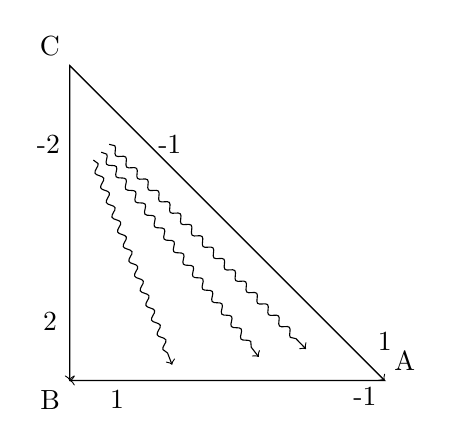
\begin{tikzpicture}
			% Define the points
			\coordinate (A) at (4,0);
			\coordinate (B) at (0,0);
			\coordinate (C) at (0,4);

			% Draw the triangle edges
			\draw[<-] (B) -- (A) node[near start, below, xshift=-0.4cm] {1};
			\draw[<-] (A) -- (C) node[near end, right] {-1};
			\draw[->] (C) -- (B) node[near start, left] {-2};

			% Draw the reverse direction labels
			\node at (3.75,-0.2) {-1};
			\node at (-0.25,.75) {2};
			\node at (4,.5) {1};

			% Label the points
			\node[above right] at (A) {A};
			\node[below left] at (B) {B};
			\node[above left] at (C) {C};

			% Draw the outline of the triangle without arrows
			\draw (A) -- (B) -- (C) -- cycle;


			% Draw squiggly flow lines
			\draw[->, decorate, decoration={snake, amplitude=.4mm, segment length=2mm, post length=1mm}] (0.5,3) -- (3,.4);
			\draw[->, decorate, decoration={snake, amplitude=.4mm, segment length=2mm, post length=1mm}] (0.4,2.9) -- (2.4,0.3);
			\draw[->, decorate, decoration={snake, amplitude=.4mm, segment length=2mm, post length=1mm}] (0.3,2.8) -- (1.3,0.2);
		\end{tikzpicture}
		\caption{Flow lines from choice of subgroup.}
		\label{fig:attracting-sets}
	\end{figure}
	Based on our choice of $1$-parameter subgroup, we have the following decomposition: \begin{align*}
		\C\P^2 & = C \coprod (\P^1 \backslash C) \coprod \P^2 \backslash \P^1
	\end{align*} One sees this decomposition by considering
	the attracting sets of the action for each fixed point. For $C$ the
	attracting set is $C$ itself, for $A$ the attracting set is the line $\P^1$,
	all the points of $\P^1$ except $C$ are attracted to $A$, and for $B$ the attracting
	set is $\P^2 \backslash \P^1$, where the $\P^1$ is the $T$-invariant curve which joins the fixed points $A$ and $C$. These cells are all affine spaces, and their
	closures are precisely $V(\tau_i) = \P^i$.
\end{example}
If $X$ is not projective, then one can subdivide cones and produce
a refinement $\Sigma'$ of $\Sigma$ so that the corresponding map \begin{align*}
	\pi: X(\Sigma') \to X(\Sigma)
\end{align*} is a surjective birational $T$-equivariant morphism and
$X(\Sigma')$ is smooth and projective. The composition \begin{align*}
	\pi_*\circ \pi^*: H^*(X(\Sigma)) \to H^*(X(\Sigma))
\end{align*} is the identity on $H^*(X(\Sigma))$ and on $H^*_T(X(\Sigma))$
and therefore $\pi^*$ is injective and $\pi_*$ is surjective.

Assembling the results of the previous sections, we obtain the following proposition.

\begin{proposition}
	For any complete smooth toric variety $X$, the cohomology ring $H^*(X)$
	is generated by the classes $[V(\tau_i)]$ of the closures of the attracting sets
	as $\Z$-module, and the equivariant cohomology ring $H^*_T(X)$ is generated
	by the classes $[V(\tau_i)]^T$ as a module over $\Lambda$.
\end{proposition}

\subsection{Danilov's theorem}
Let \( D_1, \ldots, D_d \) be the \( T \)-invariant divisors, \( D_i = V(\rho_i) \) for rays \( \rho_1, \ldots, \rho_d \) of \( \Sigma \). Let \( v_i \in N \) be the minimal generator of the ray \( \rho_i \). For \( u \in M \), the element \( e^u \in \mathbb{C}[M] \) determines a rational function on \( X \). The corresponding divisor is
\[
	\operatorname{div}(e^u) = \sum_i \langle u, v_i \rangle D_i.
\]
Equivariantly, \( e^u \) is a rational section of the line bundle \( L_u \) with character \( u \), so we have a relation
\[
	u = c_1^T(L_u) = \left[\operatorname{div}(e^u)\right]^T = \sum_i \langle u, v_i \rangle [D_i]^T
\]
in \( H_T^2 X \).

Moreover given distinct rays \( \rho_{i_1}, \ldots, \rho_{i_r} \), we have
\[
	[D_{i_1}]^T \cdots [D_{i_r}]^T = [V(\tau)]^T
\]
if the rays span a cone \( \tau \) of \( \Sigma \),  zero otherwise.
Let \( X_1, \ldots, X_d \) be variables, one for each ray of the fan \( \Sigma \). Consider the following ideals
in \( \mathbb{Z}[X] = \mathbb{Z}[X_1, \ldots, X_d] \)
\begin{itemize}
	\item \( I \) is generated by all monomials \( X_{i_1} \cdots X_{i_r} \), such that the corresponding rays \( \rho_{i_1}, \ldots, \rho_{i_r} \) do not span a cone.
	\item \( J \) is generated by all elements \( \sum \langle u, v_i \rangle X_i \), ranging over all \( u \in M \).
\end{itemize}
The ring \( \mathbb{Z}[X] / I \) is called the \emph{Stanley-Reisner ring} of \( \Sigma \).

We have a homomorphism
\[
	\mathbb{Z}[X] / (I + J) \to H^*_T X,
\]
given by \( X_i \mapsto [D_i] \). Indeed, we have seen that \( I \) and \( J \) map to zero, so the homomorphism is well-defined. It is surjective, because
\[
	[V(\tau)] = [D_{i_1}] \cdots [D_{i_r}]
\]
where \( \rho_{i_1}, \ldots, \rho_{i_r} \) are the rays spanning \( \tau \). In fact, it is an isomorphism, and one deduces this from the corresponding equivariant statement.

In equivariant cohomology, we have two ideals in \( \Lambda[X] = \Lambda[X_1, \ldots, X_d] \):
\begin{itemize}
	\item \( I' \) has the same generators as \( I \), all monomials \( X_{i_1} \cdots X_{i_r} \), such that the corresponding rays \( \rho_{i_1}, \ldots, \rho_{i_r} \) do not span a cone.
	\item \( J' \) is generated by elements \( u - \sum \langle u, v_i \rangle X_i \), ranging over all \( u \in M \) (or a basis for \( M \)).
\end{itemize}

We have a homomorphism
\[
	\Lambda[X] / (I' + J') \to H^*_T X,
\]
by \( X_i \mapsto [D_i]^T \). Again, we have seen that \( I' \) and \( J' \) map to zero, so the homomorphism is well-defined; it is surjective for similar reasons. We will see that it is an isomorphism.

\begin{theorem}[Danilov]
	For any complete smooth toric variety \( X = X(\Sigma) \), we have isomorphisms of cohomology rings
	\[
		H^*X \cong \mathbb{Z}[X] / (I + J) \quad \text{and} \quad H_T^*X \cong \Lambda[X] / (I' + J').
	\]
\end{theorem}
This also identifies the equivariant cohomology of \( X = X(\Sigma) \) with the Stanley-Reisner ring of \( \Sigma \) because the canonical homomorphism
\[
	\mathbb{Z}[X] / I \to \Lambda[X] / (I' + J')
\]
is an isomorphism.
\begin{proof}
	We sketch a proof of Danilov's theorem using the GKM relations, see \cite{fulton-anderson}. For any cone \( \tau \subseteq N_\mathbb{R} \), one has the sublattice \( N_\tau \subseteq N \) spanned by \( \tau \), with corresponding quotient lattice \( M \to M_\tau \). For \( \gamma \subseteq \tau \), there is a corresponding projection \( M_\tau \to M_\gamma \). We will write \( f \mapsto f|_\gamma \) for the corresponding map \( \mathrm{Sym}^* M_\tau \to \mathrm{Sym}^* M_\gamma \). For any rational polyhedral fan \( \Sigma \) in \( N \), the ring of \emph{piecewise polynomial functions} with respect to \( \Sigma \) is
	\[
		PP^*(\Sigma) = \left\{ (f_\tau)_{\tau \in \Sigma} \mid f_\tau \in \mathrm{Sym}^* M_\tau, \text{ and } f_\tau|_\gamma = f_\gamma \text{ for all } \gamma \subseteq \tau \right\}.
	\]
	When \( \Sigma \) is a complete fan, \( PP^*(\Sigma) \) is the ring of continuous functions on \( N_\mathbb{R} \) which are given by polynomials in \( \Lambda = \mathrm{Sym}^* M \) on each maximal cone \( \sigma \). Then there are canonical isomorphisms
	\[
		\mathbb{Z}[X]/I \cong PP^*(\Sigma)
		\cong \left\{ (f_\sigma)_{\dim \sigma = n} \mid f_\sigma|_\tau = f_{\sigma'}|_\tau \text{ if } \tau \text{ is a facet of } \sigma \text{ and } \sigma' \right\}.
	\]


	By computing the characters on the \( T \)-invariant curves \( V(\tau) \), we can identify this ring with the subring of
	\[
		H_T^*X^T = \bigoplus_{\dim \sigma = n} \Lambda
	\]
	defined by the GKM conditions. It follows that \( \mathbb{Z}[X]/I \cong PP^*(\Sigma) \cong H_T^*X \).
\end{proof}
